% !TEX root = ../linal_lecture_01.tex

\begin{frame} % название фрагмента

\videotitle{Прямая, порожденная вектором, гиперплоскость} % Порожденные вектором

\end{frame}


\begin{frame}{Краткий план:}

\begin{itemize}[<+->]
  \item Да будет больше разных расстояний!
  \item Делаем из вектора прямую.
  \item Делаем из вектора гиперплоскость.
  % Ядерные функции из скалярного произведения. - в упражнения!
\end{itemize}

\end{frame}


\begin{frame}{Больше метрик в студию!}

 \begin{block}{Определение} 
 \alert{Манхэттэнская метрика} или \alert{расстояние по-Майкопски}:
  \[
  d(\ba, \bb) = \abs{a_1 - b_1}  + \abs{a_2 - b_2} + \ldots + \abs{a_n - b_n}
  \]
 \end{block}

\end{frame}




\begin{frame}{У них — Манхэттэн}
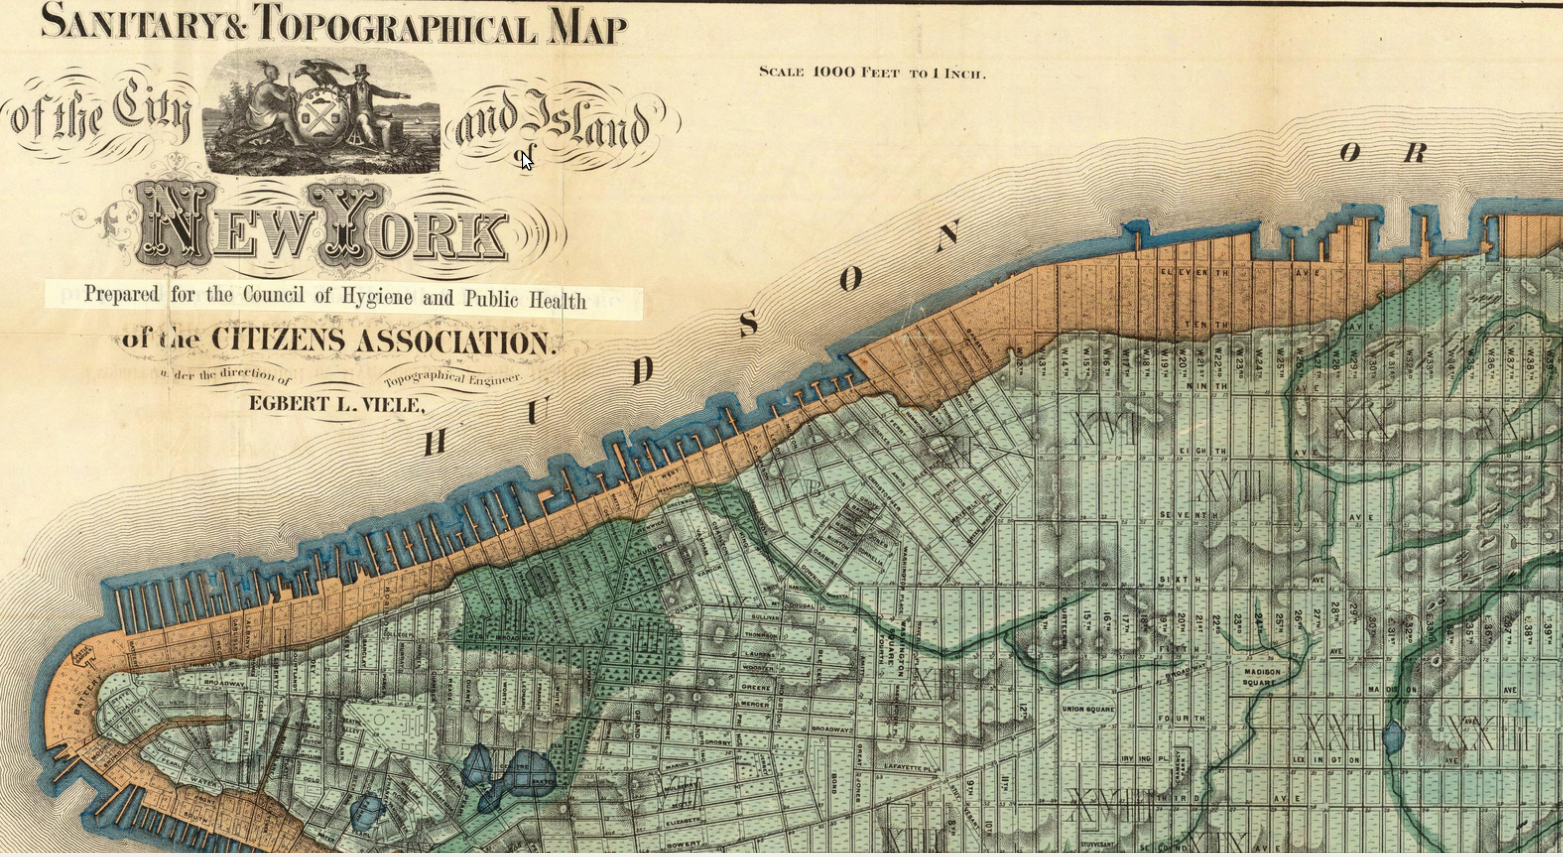
\includegraphics[scale=0.5]{figures/video_010_manhattan.png}

% \figcaption{План Манхэттэна}

\graylink{wikipedia.org / общественное достояние}
\end{frame}



\begin{frame}{У нас — Майкоп}
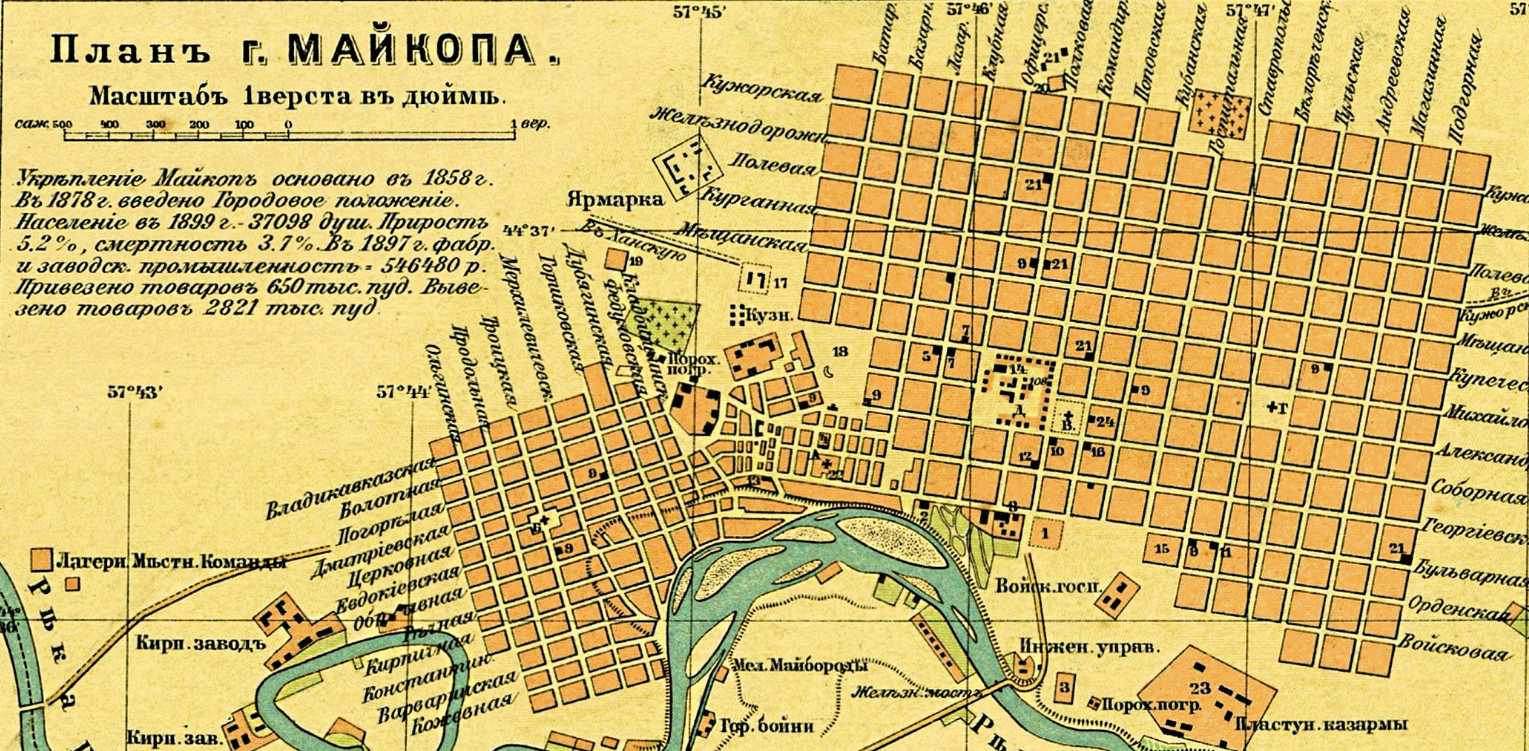
\includegraphics[scale=0.5]{figures/video_010_maykop.png}

% \figcaption{План Майкопа}

\graylink{wikipedia.org / общественное достояние}
    

\end{frame}





\begin{frame}{Ещё больше метрик!}
%\begin{block}{Метрика Чебышёва}
%  \[
%      d(a, b) = \max\left\{\abs{a_1 - b_1}, \abs{a_2 - b_2}, \ldots, \abs{a_n - b_n}\right\}
%  \]
%\end{block}

\begin{block}{Определение} 

\alert{Метрика Минковского}
  \[
      d_p(\ba, \bb) = \left(\sum_{i=1}^n \abs{a_i - b_i}^p \right)^{1/p}
  \]
\end{block}
\end{frame}

\begin{frame}{Частные случаи метрики Минковского}

  
\alert{Евклидова метрика, $p=2$}
$
   d_2(\ba, \bb) = \sqrt{(a_1 - b_1)^2 + \ldots + (a_n - b_n)^2} 
$

\alert{Манхэттэнская метрика, $p=1$}
$
d_1(\ba, \bb) = \abs{a_1 - b_1}  + \abs{a_2 - b_2} + \ldots + \abs{a_n - b_n} 
$

%\begin{block}{Метрика Чебышёва, $p\to \infty$}
%$
    %\max\left\{\abs{a_1 - b_1}, \ldots, \abs{a_n - b_n}\right\} = \lim_{p\to\infty} d_p(a, b)
%$
%\end{block}

\begin{center}
\begin{tikzpicture}[
scale=1.8,
MyPoints/.style={draw=blue,fill=white,thick},
Segments/.style={draw=blue!50!red!70,thick},
MyCircles/.style={green!50!blue!50,thin}, 
every node/.style={scale=1.2}
]

\draw[color=gray,step=1.0,dotted] (-1.1,-2.1) grid (7.6,5.1);
%\grid;


%%\draw[->, >=stealth] (-1,0)--(6.5,0) node[right]{$x_1$};
%\draw[-{Latex[length=4.5mm, width=2.5mm]}, >=stealth] (0,-1)--(0,5) node[above left]{$x_2$};
%
%\draw[-{Latex[length=4.5mm, width=2.5mm]}, >=stealth] (-1,0)--(6.5,0) 
%node[right]{$x_1$};

% Feel free to change here coordinates of points A and B
\pgfmathparse{0}		\let\Xa\pgfmathresult
\pgfmathparse{0}		\let\Ya\pgfmathresult
\coordinate (A) at (\Xa,\Ya);

\pgfmathparse{1}		\let\Xb\pgfmathresult
\pgfmathparse{4}		\let\Yb\pgfmathresult
\coordinate (B) at (\Xb,\Yb);

\pgfmathparse{5}		\let\Xc\pgfmathresult
\pgfmathparse{1}		\let\Yc\pgfmathresult
\coordinate (C) at (\Xc,\Yc);

\pgfmathparse{5}		\let\Xd\pgfmathresult
\pgfmathparse{4}		\let\Yd\pgfmathresult
\coordinate (D) at (\Xd,\Yd);




% Let I be the midpoint of [AB]
\pgfmathparse{(\Xb+\Xa)/2} \let\XI\pgfmathresult
\pgfmathparse{(\Yb+\Ya)/2} \let\YI\pgfmathresult
\coordinate (I) at (\XI,\YI);	


\draw[-{Latex[length=4.5mm, width=2.5mm]}, >=stealth, darkgray,thick] (A)--(B) node[midway,left]{$\ba$};


\draw[-{Latex[length=4.5mm, width=2.5mm]}, >=stealth, darkgray,thick] (A)--(C) node[midway,below]{$\bb$};

\draw[veca,thick, line width=0.35mm] (D)--(B);
\draw[veca,thick, line width=0.35mm] (C)--(D);


\draw[vecb,thick, line width=0.35mm] (C)--(B) node[midway,below left ]{$d_2(\ba,\bb)$};

\draw[vecc,thick, line width=0.35mm] (C) to[bend right] (B);

\node [above, vecc] at (4,3) {$d_p(\ba,\bb)$};



\node [above right, veca] at (4, 4) {$d_1(\ba,\bb)$}; 

\end{tikzpicture}
\end{center}
    


\end{frame}





\begin{frame}{Вектор порождает прямую}

\begin{block}{Определение} 
\alert{Прямая порождённая вектором $a$}, $\Span a$

Множество векторов, получаемых при домножении вектора $a$ на произвольное число,
\[
\Span \ba = \left\{t\cdot \ba \middle| t \in \R \right\}  
\]
\end{block}

\pause

\begin{center}

\begin{tikzpicture}[
scale=1.2,
MyPoints/.style={draw=blue,fill=white,thick},
Segments/.style={draw=blue!50!red!70,thick},
MyCircles/.style={green!50!blue!50,thin}, 
every node/.style={scale=1.2}
]
%\grid;
\clip (-1.5,-1.5) rectangle (5.5,5.5);

\pgfmathparse{1}		\let\Xa\pgfmathresult
\pgfmathparse{1}		\let\Ya\pgfmathresult
\coordinate (A) at (\Xa,\Ya);

\pgfmathparse{3}		\let\Xb\pgfmathresult
\pgfmathparse{3}		\let\Yb\pgfmathresult
\coordinate (B) at (\Xb,\Yb);

\pgfmathparse{5}		\let\Xc\pgfmathresult
\pgfmathparse{5}		\let\Yc\pgfmathresult
\coordinate (C) at (\Xc,\Yc);

\pgfmathparse{-1}		\let\Xd\pgfmathresult
\pgfmathparse{-1}		\let\Yd\pgfmathresult
\coordinate (D) at (\Xd,\Yd);



\draw[ black,dashed] (D)--(C); % node[above left]{$\Span \ba$};

\draw[-{Latex[length=4.5mm, width=2.5mm]}, >=stealth, veca,thick] (A)--(B) node[midway,above left]{$\ba$};


\end{tikzpicture}
\end{center}


\end{frame}





\begin{frame}{Вектор задаёт гиперплоскость}

Вектор $\ba$ фиксирован, например, $\ba=(1, 2)$.

%\begin{block}{TODO: две картинки рядом}
%$\langle \ba, \bv \rangle = 0$ и $\langle \ba, \bv \rangle = 1$   
%\end{block}


\begin{minipage}{0.45\textwidth}
    
\begin{tikzpicture}[
scale=1.2,
MyPoints/.style={draw=blue,fill=white,thick},
Segments/.style={draw=blue!50!red!70,thick},
MyCircles/.style={green!50!blue!50,thin}, 
every node/.style={scale=1.2}
]
%\grid;
\clip (-1.5,-1.5) rectangle (5.5,6.5);

\pgfmathparse{2}		\let\Xa\pgfmathresult
\pgfmathparse{2}		\let\Ya\pgfmathresult
\coordinate (A) at (\Xa,\Ya);

\pgfmathparse{4}		\let\Xb\pgfmathresult
\pgfmathparse{4}		\let\Yb\pgfmathresult
\coordinate (B) at (\Xb,\Yb);

\pgfmathparse{-1}		\let\Xc\pgfmathresult
\pgfmathparse{5}		\let\Yc\pgfmathresult
\coordinate (C) at (\Xc,\Yc);

\pgfmathparse{5}		\let\Xd\pgfmathresult
\pgfmathparse{-1}		\let\Yd\pgfmathresult
\coordinate (D) at (\Xd,\Yd);

\pgfmathparse{0}		\let\Xe\pgfmathresult
\pgfmathparse{4}		\let\Ye\pgfmathresult
\coordinate (E) at (\Xe,\Ye);



\draw[ black,dashed] (D)--(C);

\draw[-{Latex[length=4.5mm, width=2.5mm]}, >=stealth, veca,thick] (A)--(B) node[midway,above left]{$\ba$};

\draw[-{Latex[length=4.5mm, width=2.5mm]}, >=stealth, vecb,thick] (A)--(E) node[midway,below left]{$\bv$};

\tkzMarkRightAngle[size=0.3](E,A,B);


\node [above right] at (1, 4.5) {$\langle \ba, \bv  \rangle = 0$}; 


\end{tikzpicture}
\end{minipage}
\hfill
\begin{minipage}{0.45\textwidth}
\begin{tikzpicture}[
scale=1.2,
MyPoints/.style={draw=black,fill=red,thick},
Segments/.style={draw=blue!50!red!70,thick},
MyCircles/.style={green!50!blue!50,thin}, 
every node/.style={scale=1.2}
]
%\grid;
\clip (-1.5,-1.5) rectangle (5.5,6.5);

\pgfmathparse{0}		\let\Xa\pgfmathresult
\pgfmathparse{0}		\let\Ya\pgfmathresult
\coordinate (A) at (\Xa,\Ya);

\pgfmathparse{3}		\let\Xb\pgfmathresult
\pgfmathparse{3}		\let\Yb\pgfmathresult
\coordinate (B) at (\Xb,\Yb);

\pgfmathparse{-1}		\let\Xc\pgfmathresult
\pgfmathparse{5}		\let\Yc\pgfmathresult
\coordinate (C) at (\Xc,\Yc);

\pgfmathparse{5}		\let\Xd\pgfmathresult
\pgfmathparse{-1}		\let\Yd\pgfmathresult
\coordinate (D) at (\Xd,\Yd);

\pgfmathparse{0}		\let\Xe\pgfmathresult
\pgfmathparse{4}		\let\Ye\pgfmathresult
\coordinate (E) at (\Xe,\Ye);

\pgfmathparse{2}		\let\Xf\pgfmathresult
\pgfmathparse{2}		\let\Yf\pgfmathresult
\coordinate (F) at (\Xf,\Yf);



\draw[ black,dashed] (D)--(C);

\draw[-{Latex[length=4.5mm, width=2.5mm]}, >=stealth, veca,thick] (A)--(B) node[below right]{$\ba$};

\draw[-{Latex[length=4.5mm, width=2.5mm]}, >=stealth, vecb,thick] (A)--(E) node[below left]{$\bv$};

\draw[veca,thick] (A)--(F) node[midway,below right]{$\frac{1}{\|\ba\|}$};



\node [above right] at (1, 4.5) {$\langle \ba, \bv  \rangle = 1$}; 

\node [below left] at (A) {$0$}; 


\fill[MyPoints] (A) circle (0.8mm);
\fill[MyPoints] (F) circle (0.8mm);


\end{tikzpicture}


\end{minipage}


$a_1 v_1 + a_2 v_2 = 0$ \hspace{8cm} $a_1 v_1 + a_2 v_2 = 1$

\end{frame}



% \begin{frame}{Ядерные функции}

% Векторная функция $f$ фиксирована, например, 
% \[
%   f : \begin{pmatrix}
%     v_1 \\
%     v_2 \\
%   \end{pmatrix} \to 
%   \begin{pmatrix}
%     -1 \\
%     v_1^2 + v_2^2 \\
%   \end{pmatrix}
% \]

% \begin{block}{Ядерная функция, ядро $K$}
% Скалярное произведение в спрямляющем пространстве:
% $K(a, b) = \langle f(a), f(b) \rangle$.
% \end{block}
% \end{frame}

% \begin{frame}
%   \frametitle{Спрямляющее пространство:}

% \begin{block}{TODO: картинка с исходным и спрямляющим пространством} 

% \end{block}


% \end{frame}

    